% ==============================================================================
% CHƯƠNG: TÍCH HỢP TRÍ TUỆ NHÂN TẠO
% ==============================================================================
\section{Tích hợp trí tuệ nhân tạo}
\label{sec:ai_integration}

% ==============================================================================
% SUBSECTION 1: TỔNG QUAN HỆ THỐNG AI
% ==============================================================================
\subsection{Tổng quan hệ thống AI}
\label{subsec:ai_overview}

\noindent\textbf{Mô tả chung:}
Module AI của đồ án được xây dựng dưới dạng một ứng dụng web độc lập, tích hợp trực tiếp vào tập dữ liệu \texttt{car\_detail.csv} với 33.848 tin đăng xe. Hệ thống cung cấp một giao diện chat cho phép người dùng đặt câu hỏi phân tích bằng ngôn ngữ tự nhiên, yêu cầu AI viết và giải thích đoạn code Python, sau đó tự quyết định có thực thi code đó hay không. Ngoài ra, hệ thống mở Public API để các ứng dụng bên ngoài có thể gọi vào sử dụng.

\noindent\textbf{Vai trò phân công giữa AI và con người:}
\begin{itemize}
    \item \textbf{AI đảm nhận:} Đề xuất hướng phân tích khi người dùng chưa có ý tưởng; tự động sinh code Python/Pandas kèm giải thích bằng ngôn ngữ tự nhiên; trình bày kết quả tính toán dưới dạng bảng Markdown, biểu đồ Matplotlib và câu nhận xét ngắn gọn từ số liệu thực trong tập dữ liệu.
    \item \textbf{Con người đảm nhận:} Đặt ra câu hỏi và hướng phân tích; đọc, chỉnh sửa tham số trong đoạn code AI vừa sinh; ra quyết định có thực thi code hay không; phê duyệt hoặc từ chối các thao tác thay đổi file.
    \item \textbf{Ràng buộc quan trọng:} Code chỉ được chạy trên môi trường local của người dùng. AI không được tự ý thay đổi dữ liệu gốc hay tự sáng tác con số ngoài tập dữ liệu được cung cấp.
\end{itemize}

\noindent\textbf{Công cụ và công nghệ sử dụng:}

% Nhớ đảm bảo \usepackage{xltabular} đã có trong preamble

{\small
\begin{xltabular}{\textwidth}{L{3.8cm} L{3.2cm} Y}
\caption{Công cụ và công nghệ sử dụng trong module AI}
\label{tab:ai_tools} \\
\hline
\textbf{Công cụ / Thư viện} & \textbf{Vai trò} & \textbf{Mô tả sử dụng trong hệ thống} \\ \hline
\endfirsthead

% Cấu hình phần đầu bảng (header) lặp lại khi sang trang mới
\multicolumn{3}{c}%
{{\bfseries Bảng \thetable\ tiếp theo từ trang trước}} \\
\hline
\textbf{Công cụ / Thư viện} & \textbf{Vai trò} & \textbf{Mô tả sử dụng trong hệ thống} \\ \hline
\endhead

% Cấu hình phần chân bảng (footer) ở các trang bị ngắt
\hline \multicolumn{3}{r}{{Tiếp tục ở trang sau...}} \\
\endfoot

% Cấu hình phần chân bảng ở trang cuối cùng
\hline
\endlastfoot

% --- Nội dung bảng ---
FastAPI (Python) & Backend API & Xây dựng ba API bắt buộc: API AI, API Thực thi và API Logs; hỗ trợ streaming SSE để trả lời theo từng token. \\
Next.js (TypeScript) & Frontend & Giao diện chat tương tác, hiển thị code editor có thể chỉnh sửa, card phê duyệt thao tác file và biểu đồ inline. \\
LangChain & Agentic Framework & Quản lý vòng lặp ReAct, liên kết LLM với 15 công cụ, xây dựng lịch sử hội thoại đa lượt. \\
Pandas / NumPy & Tính toán dữ liệu & Thực thi truy vấn phân tích trực tiếp trên DataFrame 33.848 dòng trong bộ nhớ, đảm bảo số liệu từ dữ liệu thực. \\
Matplotlib / Seaborn & Trực quan hóa & Vẽ biểu đồ từ code do AI sinh, tự động encode thành base64 và hiển thị inline trên giao diện chat. \\
Groq / OpenAI / Google / Ollama & Nhà cung cấp LLM & Bốn provider AI có thể hoán đổi từ giao diện quản trị; hỗ trợ cả mô hình đám mây lẫn mô hình local. \\
Playwright + BeautifulSoup & Scraping Agent & Thu thập thông số kỹ thuật và giá xe từ URL người dùng cung cấp, ghi kết quả ra file JSON hoặc CSV. \\
\end{xltabular}
}

\begin{figure}[H]
\centering
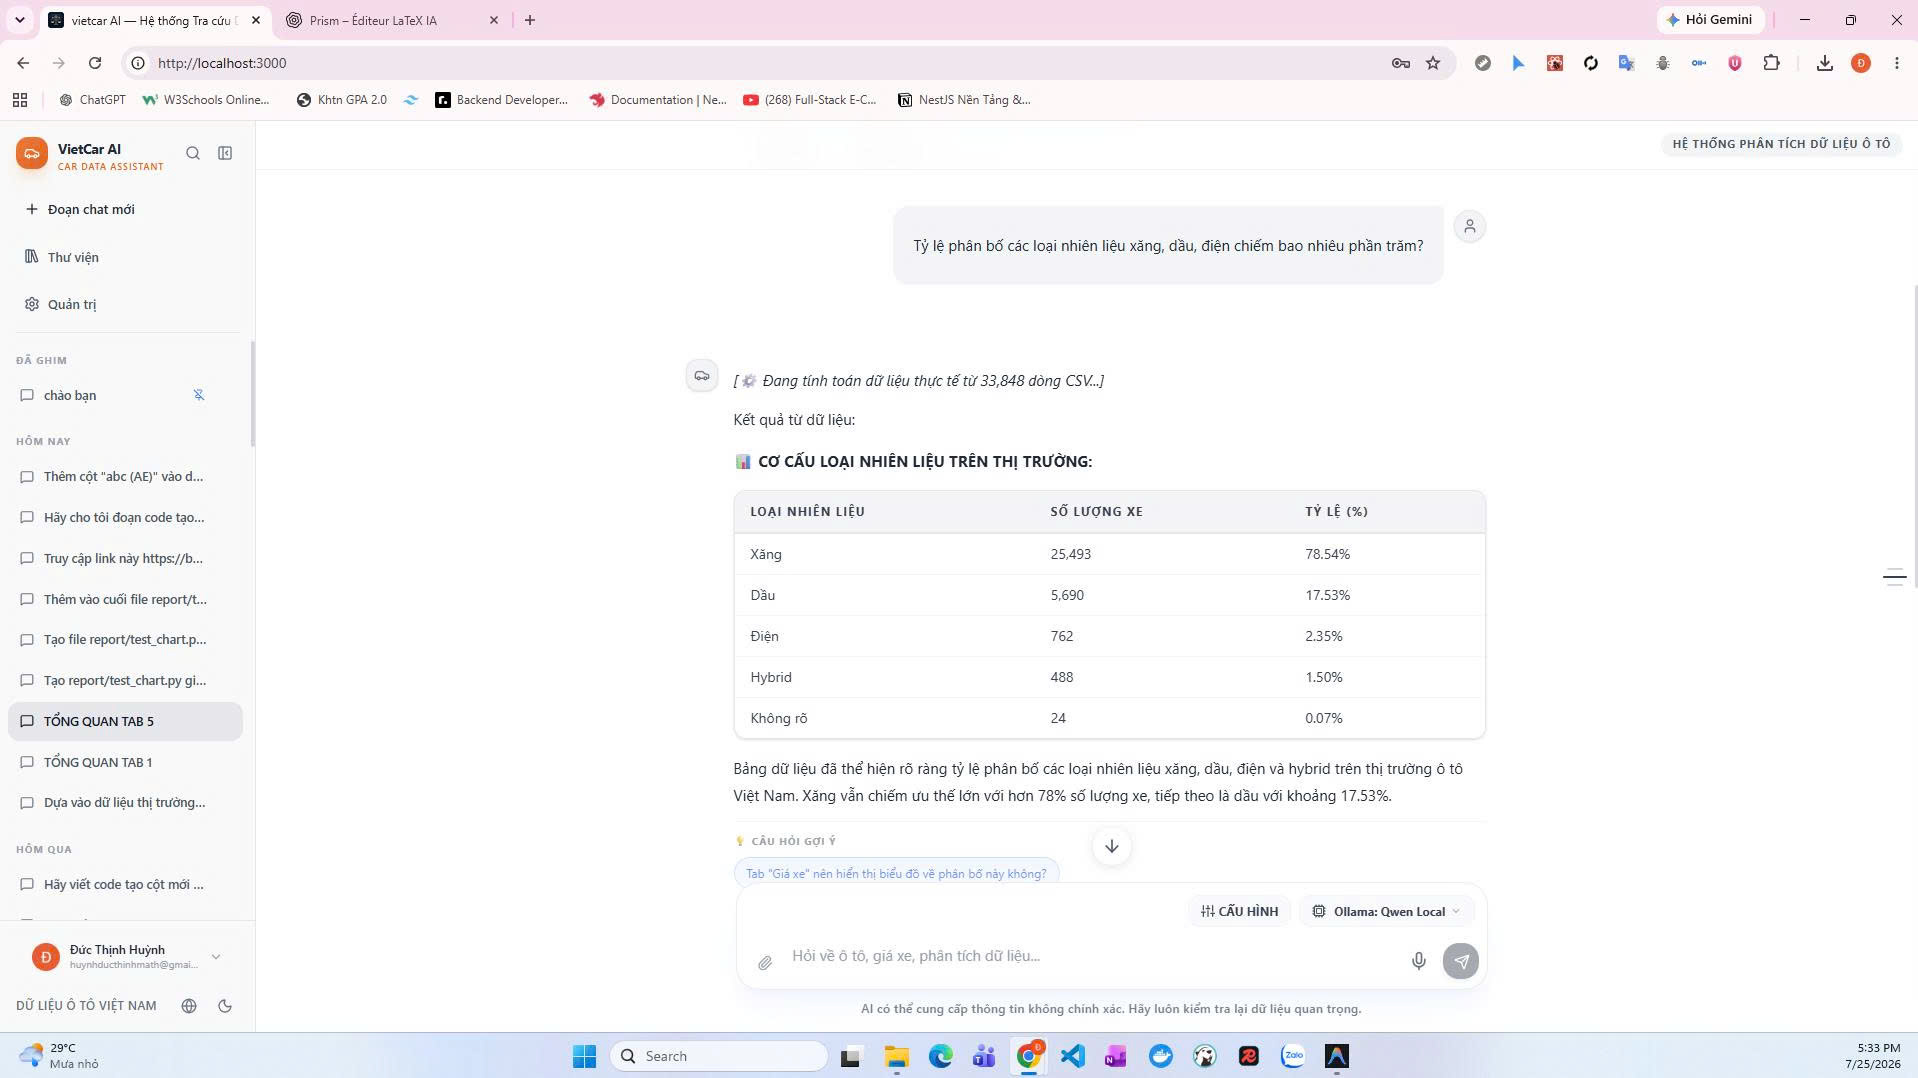
\includegraphics[width=1.00\textwidth]{graphics/AI/ai_overview.jpg}
\caption{Giao diện chính của module AI - ô chat nhận yêu cầu, vùng hiển thị kết quả và lịch sử phiên hội thoại.}
\label{fig:ai_chat_overview}
\end{figure}

% ==============================================================================
% SUBSECTION 2: KIẾN TRÚC KỸ THUẬT
% ==============================================================================
\subsection{Kiến trúc kỹ thuật}
\label{subsec:ai_architecture}

\noindent\textbf{Kiến trúc tổng thể:}
Hệ thống được tổ chức theo mô hình client -- server hai tầng. Tầng Frontend (Next.js, cổng 3000) chịu trách nhiệm thu nhận yêu cầu người dùng và hiển thị kết quả. Tầng Backend (FastAPI, cổng 8000) xử lý toàn bộ logic AI, tính toán dữ liệu và quản lý file, sau đó trả kết quả về Frontend qua giao thức HTTP hoặc SSE Streaming.

\begin{table}[H]
\centering
\small
\begin{tabularx}{\textwidth}{L{3.8cm} L{5.5cm} Y}
\textbf{Router / Module} & \textbf{Endpoint chính} & \textbf{Chức năng} \\ \hline
\texttt{analysis\_chat.py} & \texttt{POST} \newline \texttt{/api/analysis/chat} & API AI: tiếp nhận yêu cầu, gọi LLM kèm ngữ cảnh dữ liệu, streaming SSE từng token. \\
\texttt{execute.py} & \texttt{POST} \newline \texttt{/api/analysis/execute} & API Thực thi: chạy code đã được người dùng phê duyệt, trả về stdout và biểu đồ. \\
\texttt{logs\_analysis.py} & \texttt{POST /log} \newline \texttt{GET /history} & API Logs: lưu và truy xuất lịch sử yêu cầu, code, kết quả theo \texttt{session\_id}. \\
\texttt{file\_operations.py} & \texttt{POST} \newline \texttt{/api/file-operations/} \newline \texttt{\{id\}/approve} & Workflow phê duyệt thao tác file theo từng \texttt{action\_id}. \\
\texttt{public\_api.py} & \texttt{/api/public} & Public endpoint cho ứng dụng bên ngoài gọi vào phân tích dữ liệu. \\
\end{tabularx}
\caption{Danh sách các router backend và chức năng}
\label{tab:ai_routers}
\end{table}

% ------------------------------------------------------------------------------
\subsubsection{API AI (Tiếp nhận yêu cầu và sinh code có giải thích)}
\label{subsubsec:api_ai}

\noindent\textbf{Mô tả chức năng:}
API AI đóng vai trò trung tâm của hệ thống. Khi người dùng gửi một câu hỏi hoặc yêu cầu phân tích, backend không chỉ đơn giản chuyển tiếp tin nhắn đến LLM mà còn đính kèm ngữ cảnh dữ liệu phong phú, giúp mô hình AI hiểu cấu trúc bài toán và giảm khả năng sinh ra thông tin không có trong dữ liệu.

\noindent\textbf{Ngữ cảnh được gửi kèm cho LLM bao gồm:}
\begin{itemize}
    \item \textbf{Schema bộ dữ liệu:} Danh sách 21 cột, kiểu dữ liệu, ý nghĩa nghiệp vụ và thống kê mô tả cơ bản (kích thước, tỷ lệ thiếu).
    \item \textbf{Trạng thái DataFrame hiện tại:} Sau mỗi lần thực thi code, hệ thống ghi lại \texttt{df\_context} (shape, dtypes, null counts) và đưa vào context lần gọi tiếp theo, giúp AI nắm được dữ liệu đang ở trạng thái nào trong phiên làm việc.
    \item \textbf{Lịch sử hội thoại:} Các lượt hỏi đáp trước trong cùng phiên, cho phép người dùng hỏi tiếp nối mà không cần lặp lại bối cảnh.
    \item \textbf{Dữ liệu Dashboard:} Khi câu hỏi liên quan đến các chỉ số KPI hoặc biểu đồ đã có trong dashboard Power BI, hệ thống trích xuất trực tiếp từ \texttt{Dashboard.json} và đưa vào phản hồi mà không cần gọi LLM tính toán lại.
\end{itemize}

\noindent\textbf{Yêu cầu đối với đầu ra của AI:}
\begin{itemize}
    \item Khi AI sinh code Python, đoạn code đó phải được hiển thị rõ ràng trong khối \texttt{InteractiveCodeBlock} trên giao diện, kèm theo đoạn giải thích bằng ngôn ngữ tự nhiên phía trên.
    \item Giải thích phải mô tả cụ thể đoạn code sẽ làm gì (ví dụ: ``Đoạn code dưới đây nhóm dữ liệu theo cột \texttt{Hãng} và tính giá trung vị cho mỗi nhóm, sau đó sắp xếp theo thứ tự giảm dần.'').
    \item AI không được tự ý thêm số liệu hay kết quả phân tích nếu chưa có đoạn code tương ứng được thực thi thành công.
\end{itemize}

% ------------------------------------------------------------------------------
\subsubsection{API Thực thi (Chạy code đã được phê duyệt trên local)}
\label{subsubsec:api_execute}

\noindent\textbf{Mô tả chức năng:}
Sau khi AI sinh ra đoạn code, người dùng có thể đọc, chỉnh sửa và quyết định có thực thi hay không. Khi bấm nút \textbf{Thực thi}, Frontend gửi đoạn code (có thể đã được người dùng sửa đổi so với bản gốc AI sinh ra) lên \texttt{POST /api/analysis/execute}. Backend thực thi code trực tiếp trên dữ liệu tại máy.

\noindent\textbf{Cơ chế namespace bền vững theo phiên:}
\begin{itemize}
    \item Mỗi phiên làm việc (\texttt{session\_id}) được cấp một namespace Python riêng, lưu giữ biến \texttt{df} và các biến khác giữa các lần thực thi. Người dùng không cần load lại dữ liệu ở mỗi câu hỏi mới trong cùng phiên.
    \item Khi phiên kết thúc hoặc hết hạn, namespace được giải phóng để thu hồi bộ nhớ.
\end{itemize}

\noindent\textbf{Xử lý kết quả trả về:}
\begin{itemize}
    \item \textbf{Văn bản (stdout):} Kết quả in ra từ \texttt{print()} hoặc giá trị cuối cùng của biểu thức được trả về và hiển thị trong khung kết quả bên dưới ô code.
    \item \textbf{Biểu đồ (hình ảnh):} Sau khi code chạy xong, hệ thống quét tất cả figure Matplotlib đang mở, encode sang định dạng PNG base64 và nhúng trực tiếp vào giao diện chat mà không cần lưu file ảnh ra đĩa.
    \item \textbf{Lỗi thực thi:} Nếu code gây ra exception, thông báo lỗi được hiển thị rõ ràng để người dùng biết và điều chỉnh.
\end{itemize}

\begin{table}[H]
\centering
\small
\begin{tabularx}{\textwidth}{L{3cm} L{3cm} Y}
\textbf{Tham số gửi lên} & \textbf{Kiểu} & \textbf{Mô tả} \\ \hline
\texttt{code} & string & Đoạn code Python người dùng muốn thực thi (có thể khác với bản AI sinh nếu đã sửa). \\
\texttt{session\_id} & string & Định danh phiên làm việc để hệ thống truy xuất đúng namespace Python tương ứng. \\ \hline
\textbf{Kết quả trả về} & & \\ \hline
\texttt{stdout} & string & Toàn bộ văn bản in ra trong quá trình thực thi. \\
\texttt{images} & list[string] & Danh sách biểu đồ dạng base64 PNG, một phần tử cho mỗi figure Matplotlib. \\
\texttt{error} & string & Thông báo lỗi nếu có exception xảy ra. \\
\texttt{df\_context} & string & Mô tả trạng thái DataFrame sau khi thực thi, được lưu để đưa vào context lần hỏi tiếp theo. \\
\end{tabularx}
\caption{Cấu trúc request và response của API Thực thi}
\label{tab:execute_api}
\end{table}
\begin{figure}[H]
\centering
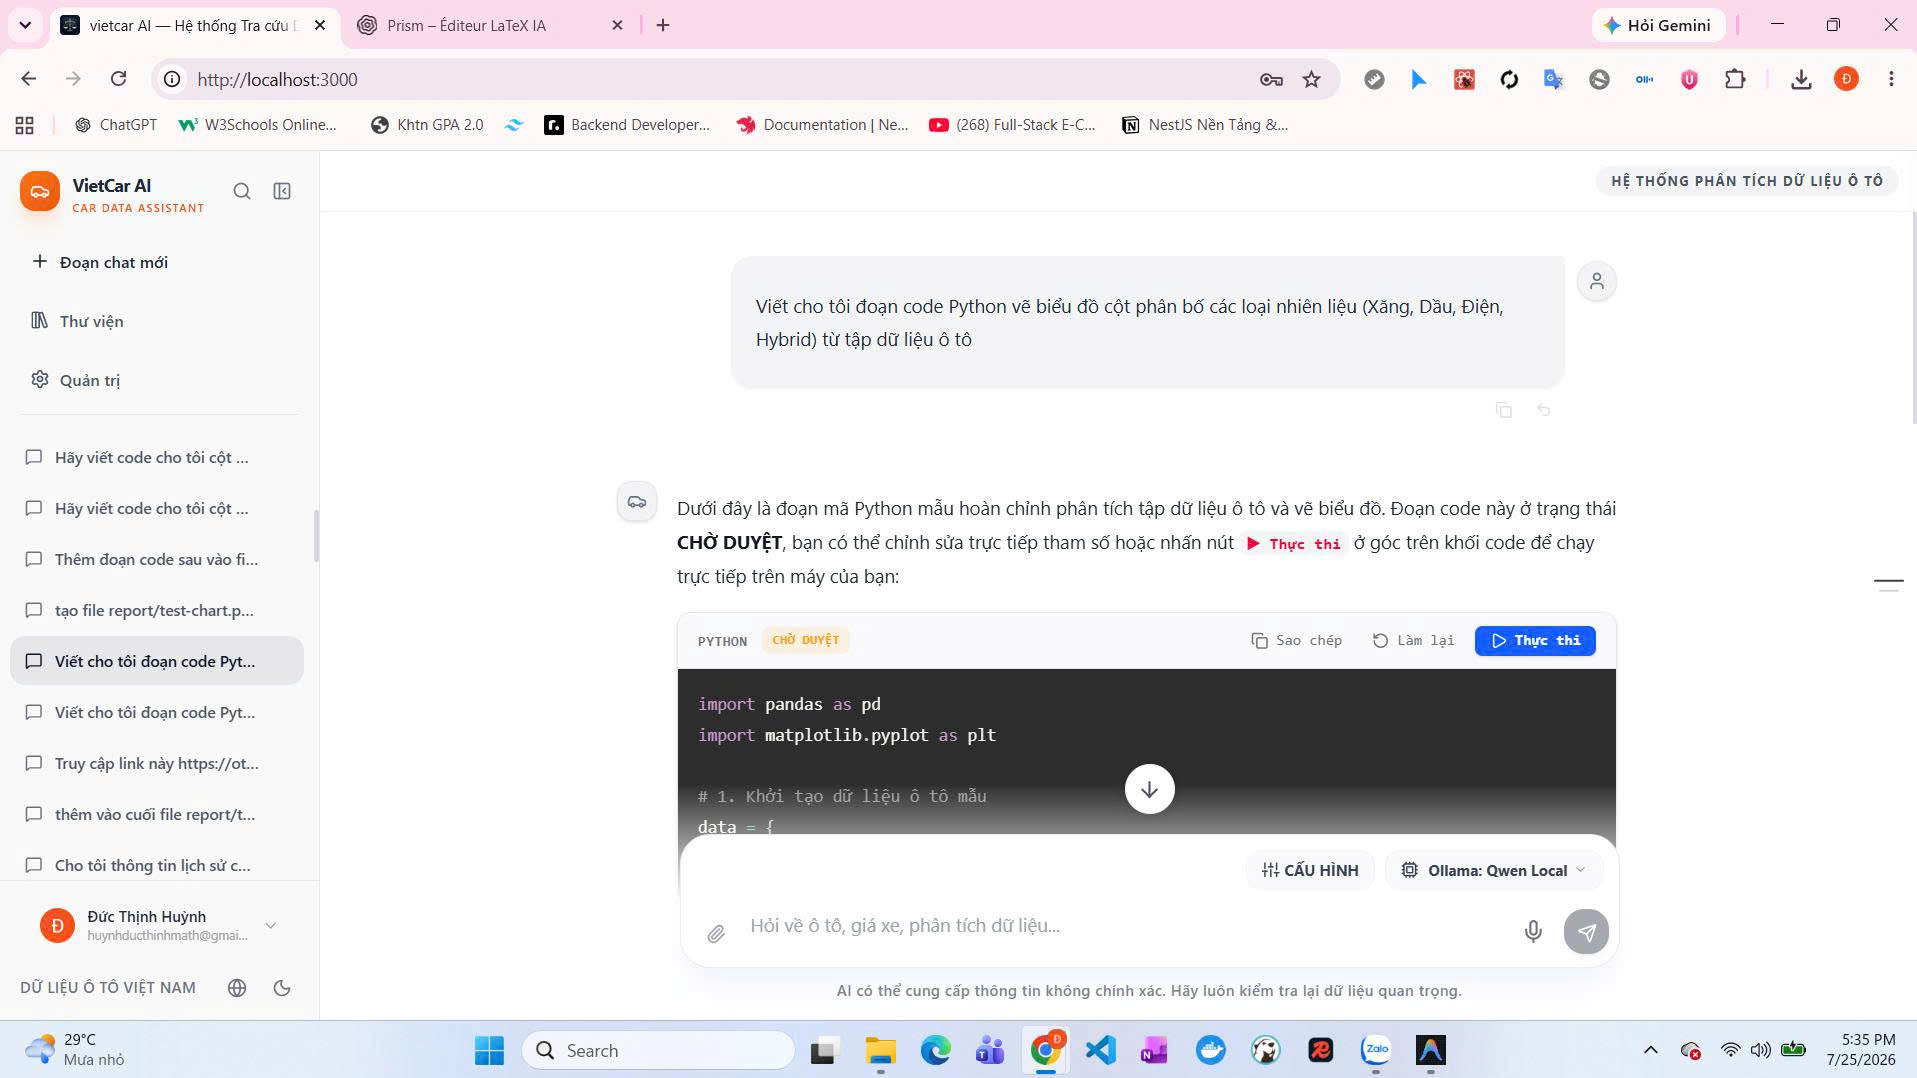
\includegraphics[width=1.00\textwidth]{graphics/AI/ai_tr79.jpg}
\caption{Khối \texttt{InteractiveCodeBlock}: editor code có thể chỉnh sửa ở trên, vùng kết quả bên dưới hiển thị bảng dữ liệu hoặc biểu đồ Matplotlib sau khi bấm Thực thi.}
\label{fig:ai_chat_overview}
\end{figure}


% ------------------------------------------------------------------------------
\subsubsection{API Logs (Lưu trữ yêu cầu, mã nguồn và kết quả)}
\label{subsubsec:api_logs}

\noindent\textbf{Mô tả chức năng:}
Theo nguyên tắc lưu trữ được quy định trong hướng dẫn tích hợp AI, hệ thống ghi lại toàn bộ nhật ký hoạt động vào file \texttt{logs/analysis\_logs.jsonl} ở định dạng JSON Lines.

\noindent\textbf{Thông tin được lưu trong mỗi bản ghi:}
\begin{itemize}
    \item \textbf{Yêu cầu người dùng:} Nội dung câu hỏi hoặc yêu cầu phân tích gốc (\texttt{user\_request}).
    \item \textbf{Mã nguồn:} Đoạn code Python AI sinh ra (\texttt{code}), phản ánh đúng trạng thái cuối cùng trước khi thực thi.
    \item \textbf{Kết quả phân tích:} Văn bản in ra từ quá trình thực thi (\texttt{execution\_result}).
    \item \textbf{Phản hồi AI:} Toàn bộ nội dung giải thích và nhận xét của AI (\texttt{ai\_response}).
    \item \textbf{Số biểu đồ:} Đếm số lượng figure Matplotlib đã được tạo ra (\texttt{charts\_count}).
    \item \textbf{Thời điểm:} Timestamp ISO 8601 của mỗi lượt tương tác.
\end{itemize}

\noindent\textbf{Truy xuất lại lịch sử:}
Endpoint \texttt{GET /history?session\_id=\{id\}\&limit=50} trả về danh sách các bản ghi theo thứ tự mới nhất trước. Người dùng có thể dùng API này để kiểm tra lại đoạn code nào đã chạy trong phiên làm việc trước hoặc trích xuất kết quả để viết báo cáo.

% ==============================================================================
% SUBSECTION 3: NGUYÊN TẮC VẬN HÀNH — HUMAN-IN-THE-LOOP
% ==============================================================================
\subsection{Nguyên tắc vận hành}
\label{subsec:ai_hitl}

\noindent\textbf{Triết lý thiết kế:}
Module AI được thiết kế theo nguyên tắc Human-in-the-Loop: AI đề xuất và trình bày, con người kiểm tra và quyết định. Không có thao tác nào tác động đến dữ liệu hoặc file dự án xảy ra mà không có sự xác nhận tường minh của người dùng.

% ------------------------------------------------------------------------------
\subsubsection{Nguyên tắc không thực thi ngầm}
\label{subsubsec:no_auto_exec}

Mọi đoạn code do AI sinh ra đều được hiển thị trong khung \texttt{InteractiveCodeBlock} trước khi chạy. Người dùng có quyền can thiệp vào code theo các cách sau trước khi quyết định thực thi:

\begin{itemize}
    \item \textbf{Đọc và kiểm tra:} Người dùng đọc code và giải thích đi kèm để xác nhận AI hiểu đúng yêu cầu.
    \item \textbf{Chỉnh sửa tham số:} Người dùng có thể thay đổi bất kỳ giá trị nào trong code (ngưỡng lọc, tên cột, khoảng thời gian, màu biểu đồ, v.v.) trực tiếp trong editor.
    \item \textbf{Chấp nhận và thực thi:} Bấm nút \textbf{Thực thi} để gửi đoạn code (đã hoặc chưa sửa) lên API Thực thi. Kết quả trả về ngay bên dưới.
    \item \textbf{Bỏ qua:} Không bấm gì, code ở lại trong editor nhưng không chạy, không ảnh hưởng đến dữ liệu hay trạng thái phiên.
\end{itemize}

Cơ chế này đảm bảo rằng AI không thể tự ý chạy bất kỳ đoạn code nào mà không có hành động tường minh từ người dùng, phù hợp với nguyên tắc ``không thực thi ngầm''.

% ------------------------------------------------------------------------------
\subsubsection{Cơ chế phê duyệt thao tác file}
\label{subsubsec:approval_workflow}

\noindent\textbf{Bối cảnh:}
Ngoài khả năng hỏi đáp và phân tích dữ liệu, module AI còn hỗ trợ người dùng quản lý file trong dự án (tạo, sửa, xóa, di chuyển file trong các thư mục được phép). Để tránh rủi ro mất dữ liệu do thao tác sai, mọi thao tác có tính chất ghi đều đi qua một vòng phê duyệt bắt buộc.

\noindent\textbf{Phân loại mức độ rủi ro:}

\begin{table}[H]
\centering
\small
\begin{tabularx}{\textwidth}{L{2.4cm} L{4.5cm} Y}
\textbf{Mức độ rủi ro} & \textbf{Loại thao tác} & \textbf{Cơ chế xử lý} \\ \hline
LOW & Đọc nội dung file, liệt kê thư mục & Thực hiện ngay, không cần phê duyệt. \\
MEDIUM & Tạo file mới, thêm nội dung vào cuối file & Hiển thị card phê duyệt, cần người dùng xác nhận. \\
HIGH & Sửa nội dung file đang có, đổi tên, di chuyển & Hiển thị card phê duyệt, tự động tạo backup trước khi thực hiện. \\
CRITICAL & Xóa file & Hiển thị card phê duyệt, kiểm tra file tồn tại trên đĩa trước khi cho phê duyệt. \\
\end{tabularx}
\caption{Phân loại mức độ rủi ro và cơ chế xử lý tương ứng}
\label{tab:risk_level}
\end{table}

\noindent\textbf{Luồng hoạt động của vòng phê duyệt:}
\begin{enumerate}
    \item AI nhận yêu cầu liên quan đến thao tác file (ví dụ: ``Sửa dòng 11 trong file docs/test\_\allowbreak chart.py'').
    \item Hệ thống kiểm tra file có tồn tại trên đĩa không; nếu không, trả về thông báo lỗi ngay mà không tạo card phê duyệt.
    \item Nếu file hợp lệ, AI tạo một \texttt{Action ID} và Frontend hiển thị \textbf{Card Phê duyệt} kèm thông tin chi tiết về thao tác sắp thực hiện.
    \item Người dùng bấm \textbf{Phê duyệt} hoặc \textbf{Từ chối}.
    \item Nếu phê duyệt: Backend tạo bản sao lưu (với thao tác HIGH/CRITICAL), sau đó thực thi thao tác và trả về kết quả.
    \item Nếu từ chối: Thao tác bị hủy, file không bị thay đổi.
\end{enumerate}

\noindent\textbf{Bảo mật đường dẫn file:}
Hệ thống chỉ cho phép truy cập các thư mục nằm trong whitelist được cấu hình sẵn (\texttt{data/}, \texttt{docs/}, \texttt{report/}, \texttt{ML/}, \texttt{notebook/}). Các file nhạy cảm như \texttt{.env}, \texttt{*.key}, \texttt{*.pem} và thư mục hệ thống bị chặn theo danh sách mẫu cấm.

% ------------------------------------------------------------------------------
\subsubsection{Cơ chế sao lưu và hoàn tác}
\label{subsubsec:backup_rollback}

\noindent\textbf{Mô tả:}
Trước khi thực hiện bất kỳ thao tác sửa, xóa hoặc di chuyển file nào, hệ thống tự động tạo một bản sao lưu (snapshot) vào thư mục \texttt{backup/} với tên file gồm timestamp chính xác đến micro-giây và tên file gốc.

\noindent\textbf{Định dạng tên bản sao lưu:}
\begin{center}
\texttt{YYYY-MM-DD\_HH-MM-SS-microsecond\_tênfile.bak}
\end{center}

\noindent\textbf{Chính sách giữ backup:}
\begin{itemize}
    \item Mỗi file được giữ tối đa 10 phiên bản; phiên bản cũ nhất bị xóa khi vượt ngưỡng.
    \item Backup quá 30 ngày được tự động dọn dẹp trong lần sao lưu tiếp theo.
    \item Toàn bộ thao tác rollback được ghi lại vào \texttt{backup/rollback\_log.jsonl}.
\end{itemize}

\noindent\textbf{Hoàn tác theo phiên bản:}
Người dùng có thể yêu cầu AI hoàn tác về phiên bản gần nhất hoặc chỉ định đúng tên file backup muốn khôi phục. Hệ thống đọc nội dung file backup, ghi đè lên file hiện tại và ghi log hoàn tác.

% ==============================================================================
% SUBSECTION 4: KIẾN TRÚC 3 TẦNG TRẢ LỜI — KIỂM SOÁT CHÍNH XÁC SỐ LIỆU
% ==============================================================================
\subsection{Kiến trúc 3 tầng trả lời}
\label{subsec:ai_3tier}

\noindent\textbf{Bối cảnh và vấn đề cần giải quyết:}
Một trong những rủi ro phổ biến khi sử dụng LLM để phân tích dữ liệu là mô hình có thể sinh ra con số không có trong dữ liệu gốc (hiện tượng thường gọi là ``ảo giác số liệu''). Để giảm thiểu rủi ro này, hệ thống không dùng LLM để tính toán trực tiếp mà chỉ dùng LLM để sinh code hoặc tổng hợp văn bản, trong khi số liệu thực tế luôn đến từ Python/Pandas chạy trên tập dữ liệu thật.

Hệ thống phân loại câu hỏi của người dùng và chọn một trong ba tầng xử lý phù hợp, cân bằng giữa tốc độ phản hồi và độ chính xác của thông tin.

\begin{table}[H]
\centering
\small
\begin{tabularx}{\textwidth}{L{1.5cm} L{3.5cm} L{3.5cm} Y}
\textbf{Tầng} & \textbf{Tên} & \textbf{Nguồn dữ liệu} & \textbf{Loại câu hỏi phù hợp} \\ \hline
1 & Pre-warmed Topic Cache & RAM - nạp sẵn khi khởi động & Tóm tắt tổng quan từng Tab Dashboard, giới thiệu từng Notebook. \\
2 & Dashboard JSON Cache & \texttt{Dashboard.json} - cache lần đọc đầu & Chi tiết biểu đồ, bảng số liệu KPI đã tổng hợp sẵn trong dashboard. \\
3 & Pandas Engine & \texttt{car\_detail\_\allowbreak processed.\allowbreak csv} - 33.848 dòng & Câu hỏi yêu cầu tính toán mới: groupby, filter, mean, median, count theo điều kiện cụ thể. \\
\end{tabularx}
\caption{So sánh ba tầng xử lý trong kiến trúc trả lời của hệ thống AI}
\label{tab:3tier_overview}
\end{table}

% ------------------------------------------------------------------------------
\subsubsection{Tầng 1 (Pre-warmed Topic Cache)}
\label{subsubsec:tier1_cache}

\noindent\textbf{Mô tả cơ chế:}
Khi server khởi động, một luồng nền chạy sau 2 giây để nạp trước 9 bản tóm tắt cố định vào từ điển \texttt{\_TAB\_PREWARMED\_CACHE} trong bộ nhớ RAM. Các chủ đề được nạp sẵn gồm file csv, 5 Tab Dashboard và 4 Notebook phân tích. Khi người dùng hỏi về một trong các chủ đề này (ví dụ: ``Tóm tắt Tab 1 cho tôi'', ``Notebook tiền xử lý làm gì?''), hệ thống nhận diện chủ đề, lấy nội dung tóm tắt từ RAM và stream ngay ra người dùng.

\noindent\textbf{Đặc điểm:}
\begin{itemize}
    \item \textbf{Thời gian phản hồi:} Khoảng 0 ms đến khi bắt đầu stream token đầu tiên, do không có I/O đọc file hay gọi API.
    \item \textbf{Phạm vi áp dụng:} Chỉ phù hợp với câu hỏi tóm tắt hoặc tổng quan. Câu hỏi yêu cầu con số chi tiết hoặc điều kiện lọc cụ thể sẽ được chuyển sang Tầng 2 hoặc 3.
    \item \textbf{Nội dung cache:} Được viết tay và cập nhật cùng với quá trình phân tích EDA, phản ánh các insight đã được kiểm chứng từ dữ liệu.
\end{itemize}

% ------------------------------------------------------------------------------
\subsubsection{Tầng 2 (Dashboard JSON Cache)}
\label{subsubsec:tier2_dashboard}

\noindent\textbf{Mô tả cơ chế:}
Tầng 2 phục vụ các câu hỏi yêu cầu thông tin chi tiết hơn tóm tắt nhưng đã được tổng hợp sẵn trong quá trình EDA. File \texttt{Dashboard.json} được xuất từ Notebook 03, chứa toàn bộ dữ liệu đầu vào cho các biểu đồ, bảng KPI và insight của 5 Tab Dashboard. File này được đọc một lần khi có truy vấn đầu tiên và lưu vào cache module-level cho các truy vấn tiếp theo.

Tool \texttt{get\_dashboard\_info(tab=``TabX'')} tìm kiếm trong file JSON theo tab được yêu cầu và trả về nội dung tương ứng. LLM nhận kết quả này và tổng hợp thành câu trả lời bằng tiếng Việt.

\noindent\textbf{Đặc điểm:}
\begin{itemize}
    \item \textbf{Thời gian phản hồi:} Khoảng 0{,}2 đến 0{,}5 giây (thời gian LLM tổng hợp văn bản), không có I/O đọc file sau lần đầu.
    \item \textbf{Phạm vi áp dụng:} Câu hỏi về biểu đồ cụ thể, chỉ số KPI, bảng số liệu đã có sẵn trong dashboard Power BI.
    \item \textbf{Cơ chế cập nhật cache:} Cache \texttt{Dashboard.json} được giữ nguyên trong suốt vòng đời tiến trình server và không có cơ chế tự reload theo \texttt{mtime}. Khi Notebook EDA được chạy lại và xuất file \texttt{Dashboard.json} mới, cần khởi động lại server để cache phản ánh thay đổi. Đây là điểm khác biệt so với cache CSV và cache Notebook metadata, vốn đều tự động làm mới theo \texttt{mtime}.
\end{itemize}

% ------------------------------------------------------------------------------
\subsubsection{Tầng 3 (Pandas Engine tính toán thực tế)}
\label{subsubsec:tier3_pandas}

\noindent\textbf{Mô tả cơ chế:}
Tầng 3 xử lý các câu hỏi yêu cầu tính toán mới trên dữ liệu, chẳng hạn ``Tính giá trung vị của xe điện theo từng hãng trong giai đoạn 2022--2025'' hay ``Có bao nhiêu xe Hatchback đã qua sử dụng có giá dưới 500 triệu?''. Hệ thống tự động sinh đoạn code Pandas tương ứng và thực thi trực tiếp trên DataFrame đang được giữ trong bộ nhớ.

\noindent\textbf{Cơ chế kiểm soát số liệu:}
\begin{enumerate}
    \item Hệ thống phát hiện câu hỏi yêu cầu tính toán thực tế và tự động sinh code Pandas tương ứng (tool \texttt{query\_dataset\_readonly}).
    \item Thực thi code trên DataFrame thực. Kết quả (bảng số liệu Markdown) được stream ra giao diện người dùng \emph{trước}.
    \item Sau khi bảng số liệu đã hiển thị, LLM mới được cho thêm 1--2 câu nhận xét ngắn bên dưới. LLM nhận được yêu cầu bắt buộc: sử dụng đúng các con số từ kết quả tính toán, không được thay đổi hay tự thêm số liệu mới.
\end{enumerate}

\noindent\textbf{Đặc điểm:}
\begin{itemize}
    \item \textbf{Thời gian phản hồi:} Khoảng 1 đến 2 giây (thực thi Pandas trên 33.848 dòng) cộng thêm thời gian LLM nhận xét.
     \item \textbf{DataFrame cache:} Tập dữ liệu được load một lần vào bộ nhớ (\texttt{\_DF\_CACHE}) và tái sử dụng cho các truy vấn tiếp theo. Trước mỗi truy vấn, hàm \texttt{\_get\_cached\_df()} gọi \texttt{os.path.getmtime()} so sánh \texttt{mtime} hiện tại với giá trị đã lưu; nếu không khớp, DataFrame được reload tự động mà không cần restart server.
    \item \textbf{Phạm vi áp dụng:} Phù hợp với bất kỳ câu hỏi nào cần số liệu chính xác theo điều kiện lọc cụ thể mà Dashboard.json không có sẵn.
\end{itemize}

\begin{table}[H]
\centering
\small
\begin{tabularx}{\textwidth}{L{4cm} L{3cm} L{2.5cm} Y}
\textbf{Loại câu hỏi ví dụ} & \textbf{Tầng xử lý} & \textbf{TTFT ước tính} & \textbf{Lý do lựa chọn} \\ \hline
``Tóm tắt Tab 3 cho tôi'' & Tầng 1 & $\approx$ 0 ms & Chủ đề được nạp sẵn trong RAM. \\
``Tab 2 có biểu đồ gì?'' & Tầng 2 & 0{,}2 -- 0{,}5 s & Thông tin đã có trong Dashboard.json. \\
``Tính giá trung vị xe điện theo từng hãng'' & Tầng 3 & 1 -- 2 s & Cần thực thi Pandas trên dữ liệu thực. \\
``Có bao nhiêu xe Ford sản xuất năm 2023?'' & Tầng 3 & 1 -- 2 s & Cần lọc và đếm theo điều kiện cụ thể. \\
\end{tabularx}
\caption{Ví dụ phân loại câu hỏi và tầng xử lý tương ứng (TTFT: thời gian đến token đầu tiên)}
\label{tab:tier_examples}
\end{table}
\begin{figure}[H]
\centering
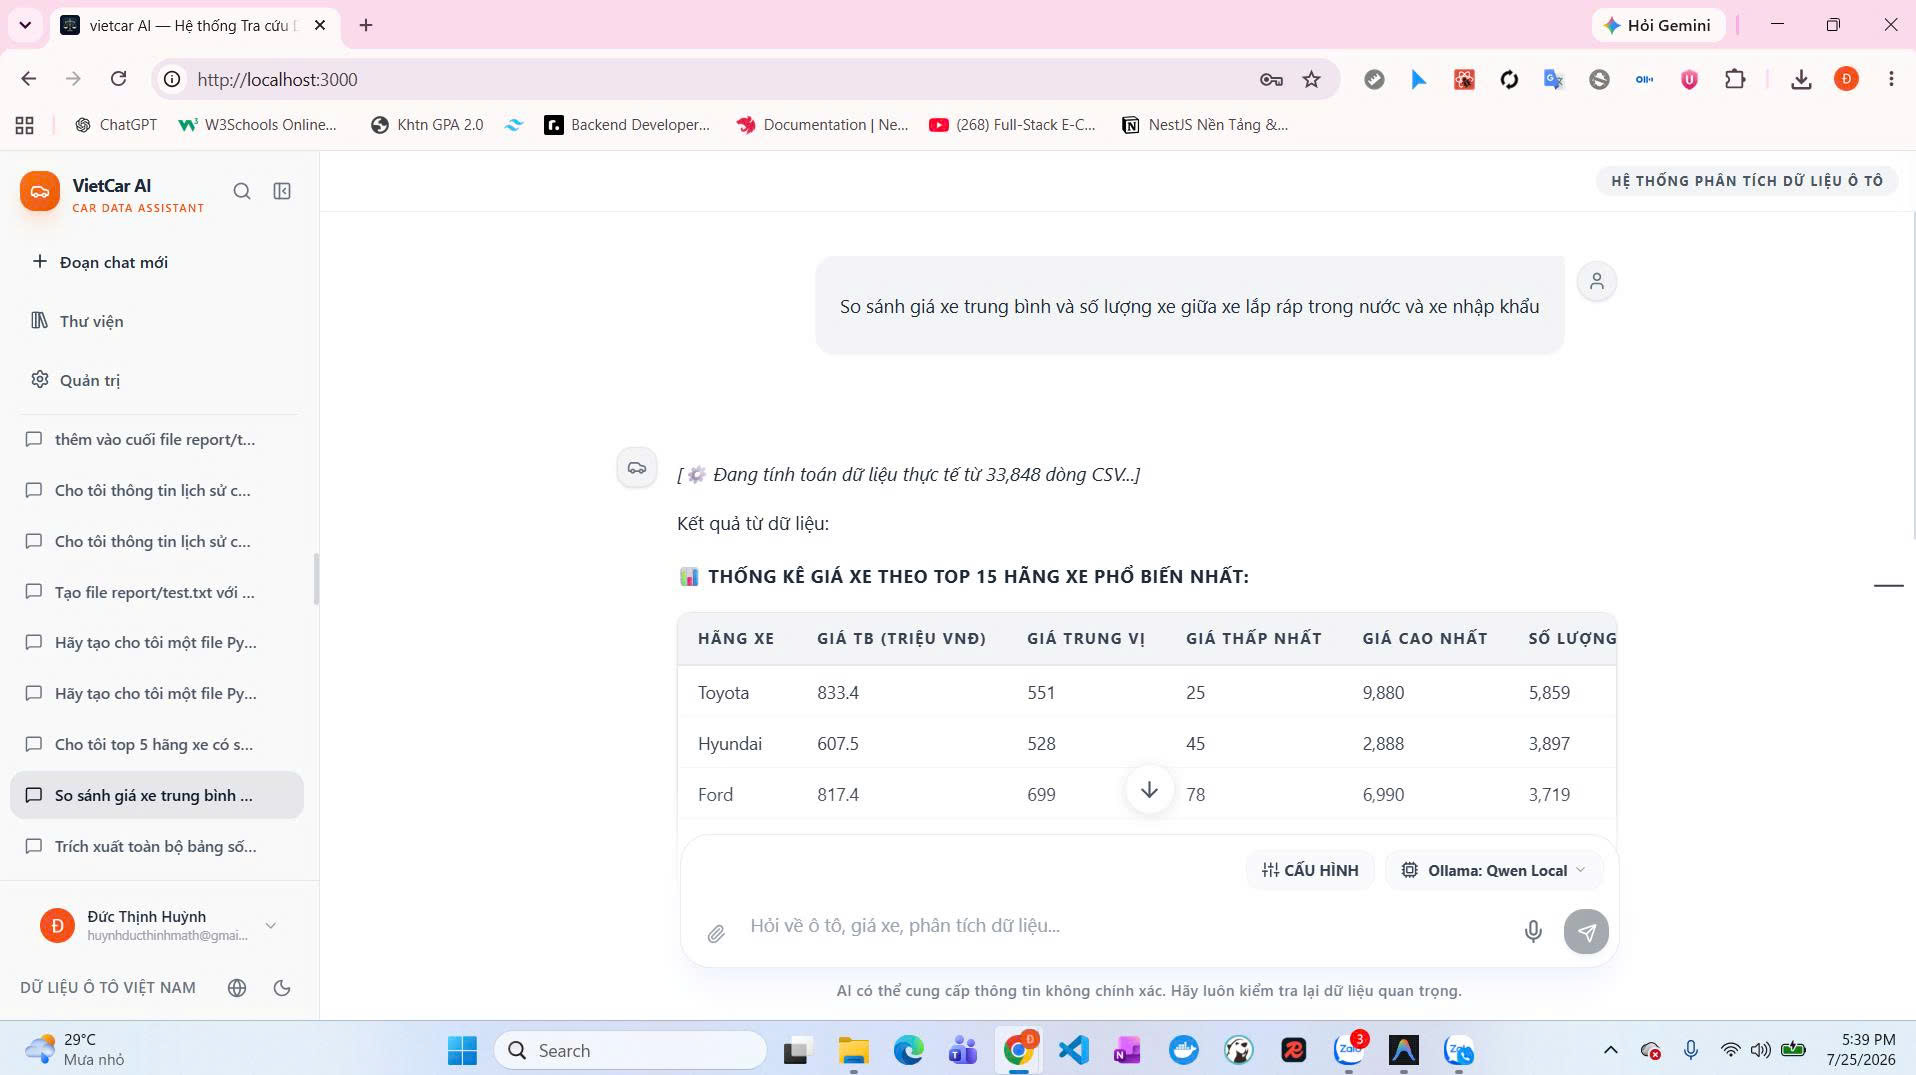
\includegraphics[width=1.00\textwidth]{graphics/AI/ai_tr86.jpg}
\caption{Phản hồi của AI khi nhận câu hỏi tính toán (Tầng 3): hiển thị thông báo ``Đang tính toán dữ liệu thực tế...'', tiếp theo là bảng Markdown số liệu chính xác, cuối cùng là 1--2 câu nhận xét ngắn của LLM bên dưới bảng.}
\label{fig:ai_chat_overview}
\end{figure}


\subsubsection{Cơ chế tự động làm mới cache khi file nguồn thay đổi}
\label{subsubsec:mtime_cache}

\noindent\textbf{Bối cảnh:}
Trong quá trình phân tích, người dùng có thể cập nhật tập dữ liệu (chạy lại notebook tiền xử lý, ghi thêm dòng từ scraping), chỉnh sửa notebook, hoặc thay đổi layout dashboard trong Power BI. Để hệ thống AI phản ánh đúng trạng thái hiện tại mà không yêu cầu thao tác thủ công, ba cơ chế theo dõi thay đổi được triển khai song song:

% Nhớ đảm bảo \usepackage{xltabular} vẫn nằm trong preamble

{\small
\begin{xltabular}{\textwidth}{L{2.8cm} L{4.5cm} L{3.5cm} Y}
\caption{Ba cơ chế tự động làm tươi cache theo loại file nguồn}
\label{tab:mtime_cache} \\
\hline
\textbf{Loại file} & \textbf{Module theo dõi} & \textbf{Cơ chế} & \textbf{Hành động khi phát hiện thay đổi} \\ \hline
\endfirsthead

% Cấu hình phần đầu bảng (header) lặp lại khi sang trang mới
\multicolumn{4}{c}%
{{\bfseries Bảng \thetable\ tiếp theo từ trang trước}} \\
\hline
\textbf{Loại file} & \textbf{Module theo dõi} & \textbf{Cơ chế} & \textbf{Hành động khi phát hiện thay đổi} \\ \hline
\endhead

% Cấu hình phần chân bảng (footer) ở các trang bị ngắt
\hline \multicolumn{4}{r}{{Tiếp tục ở trang sau...}} \\
\endfoot

% Cấu hình phần chân bảng ở trang cuối cùng
\hline
\endlastfoot

% --- Nội dung bảng ---
File CSV \newline (\texttt{.csv}) & \texttt{analysis\_chat.py} \newline — \texttt{\_get\_cached\_df()} & So sánh \texttt{mtime} trước mỗi truy vấn & Reload toàn bộ DataFrame vào RAM; các truy vấn sau dùng dữ liệu mới ngay lập tức. \\
File Notebook \newline (\texttt{.ipynb}) & \texttt{analysis\_chat.py} \newline — \texttt{\_get\_notebook\_metadata()} & So sánh \newline \texttt{dict\{path: mtime\}} của tất cả \texttt{.ipynb} & Reset cache metadata notebook; đọc lại số cell, mô tả và cấu trúc của tất cả notebook trong thư mục. \\
File Power BI \newline (\texttt{.pbix}) & \texttt{pbix\_watcher.py} \newline — thread daemon & Watchdog filesystem event; fallback poll \texttt{mtime} mỗi 10~giây & Giải nén \texttt{Report/Layout} từ ZIP, so sánh diff trang/visual; ghi log 5 thay đổi gần nhất vào context AI. \\
\end{xltabular}
}

\noindent\textbf{Chi tiết cơ chế theo dõi file .pbix:}
File \texttt{.pbix} của Power BI thực chất là một file ZIP chứa nhiều tài nguyên bên trong, trong đó có \texttt{Report/Layout} là file JSON mô tả cấu trúc tất cả các trang và visual. Service \texttt{pbix\_watcher.py} chạy trong một luồng nền riêng (daemon thread), ưu tiên dùng thư viện \texttt{watchdog} để nhận sự kiện filesystem ngay khi file được ghi. Nếu \texttt{watchdog} không khả dụng, service tự động chuyển sang chế độ polling \texttt{mtime} 10 giây một lần. Khi phát hiện thay đổi, hệ thống:
\begin{enumerate}
    \item Đọc lại file \texttt{.pbix} và giải nén \texttt{Report/Layout} JSON.
    \item So sánh với snapshot cũ: phát hiện trang mới/xóa, visual mới/xóa, thay đổi loại biểu đồ, đổi tiêu đề, thay đổi vị trí hoặc kích thước.
    \item Ghi log thay đổi vào danh sách nội bộ (giữ tối đa 20 mục).
    \item Cung cấp tóm tắt Markdown của 5 thay đổi gần nhất qua hàm \texttt{get\_summary\_for\_\allowbreak context()}, để tích hợp vào ngữ cảnh AI cho các cuộc hội thoại tiếp theo.
\end{enumerate}

\noindent\textbf{Ý nghĩa thực tế:}
Nhờ ba cơ chế này, người dùng có thể làm việc song song: chạy lại notebook, cập nhật dashboard Power BI, hoặc ghi thêm dữ liệu từ scraping trong khi cửa sổ chat AI vẫn mở và hệ thống sẽ phản ánh trạng thái mới nhất mà không cần thao tác thêm. Ngoại lệ duy nhất là cache \texttt{Dashboard.json} (Tầng 2) không được theo dõi tự động do không có cơ chế \texttt{mtime} tương ứng, và cần khởi động lại server khi file này thay đổi.


% ==============================================================================
% SUBSECTION 5: LUỒNG AGENTIC AI VÀ BỘ CÔNG CỤ
% ==============================================================================
\subsection{Luồng Agentic AI và bộ công cụ}
\label{subsec:ai_agentic}

\noindent\textbf{Mô tả chung:}
Ở cấp độ cao hơn so với mô hình hỏi đáp thông thường, module AI của đồ án vận hành theo kiến trúc Agentic. Thay vì chỉ sinh ra một câu trả lời từ câu hỏi của người dùng, AI có thể tự quyết định gọi công cụ nào, lấy dữ liệu từ nguồn nào, và lặp lại vòng đó nhiều lần trước khi tổng hợp câu trả lời cuối cùng.

% ------------------------------------------------------------------------------
\subsubsection{Cơ chế vòng lặp ReAct}
\label{subsubsec:react_loop}

Vòng lặp ReAct (Reason -- Act) là cơ chế lõi điều phối hành vi của AI Agent. Toàn bộ quá trình chia làm hai giai đoạn:

\begin{itemize}
    \item \textbf{Giai đoạn A - Lập luận và gọi công cụ (ẩn với người dùng):}
    LLM nhận câu hỏi và danh sách công cụ có sẵn, tự quyết định có cần gọi công cụ nào không và gọi với tham số gì. Nếu có \texttt{tool\_calls} trong phản hồi, hệ thống thực thi công cụ, thu kết quả, đưa kết quả vào lịch sử hội thoại và cho LLM tiếp tục suy luận. Vòng lặp này lặp lại tối đa 5 lần để tránh chạy vô hạn.
    \item \textbf{Giai đoạn B - Stream câu trả lời cuối (hiện ra người dùng):}
    Khi LLM không còn \texttt{tool\_calls} trong phản hồi, hệ thống bắt đầu stream từng token ra giao diện. Người dùng thấy câu trả lời xuất hiện dần, không phải đợi toàn bộ xử lý xong mới hiện.
\end{itemize}

\noindent\textbf{Bộ phát hiện intent nhanh (\texttt{\_detect\_direct\_tool}):}
Trước khi đưa câu hỏi vào vòng lặp ReAct đầy đủ, hệ thống chạy một bước phân loại nhanh để nhận diện các câu hỏi có thể xử lý ngay mà không cần LLM quyết định. Nếu phát hiện URL trong câu hỏi, hệ thống kích hoạt ngay Scraping Agent. Nếu câu hỏi chứa từ khóa tính toán (giá trung bình, đếm, thống kê, phân bố, v.v.), hệ thống chuyển thẳng sang Pandas Engine (Tầng 3). Nếu câu hỏi hỏi về một Tab cụ thể, hệ thống định tuyến sang Tầng 1 hoặc 2. Cơ chế này giúp rút ngắn thời gian phản hồi cho các câu hỏi phổ biến, đồng thời giảm tải gọi LLM không cần thiết.

\noindent\textbf{Cơ chế thoát vòng lặp sớm:}
Đối với các công cụ tác động đến file hoặc chạy script (tạo, sửa, xóa file, rollback, thực thi file Python, cào dữ liệu), ngay sau khi công cụ trả về kết quả, hệ thống stream kết quả ra người dùng và kết thúc vòng lặp ngay lập tức thay vì tiếp tục cho LLM xử lý thêm. Điều này tránh trường hợp vòng lặp chạy thêm nhiều lần không cần thiết sau khi thao tác đã hoàn thành.

% ------------------------------------------------------------------------------
\subsubsection{Bộ công cụ của AI Agent}
\label{subsubsec:ai_tools}

\noindent\textbf{Tổng quan:}
AI Agent được trang bị 15 công cụ, chia thành ba nhóm chức năng chính: truy vấn và phân tích dữ liệu, quản lý file trong dự án, và điều phối tác vụ phức tạp.

% Đừng quên thêm \usepackage{xltabular} vào phần preamble

{\small
\begin{xltabular}{\textwidth}{L{4.5cm} L{2.8cm} Y}
\caption{Danh sách 15 công cụ của AI Agent và chức năng tương ứng}
\label{tab:ai_tools_15} \\
\hline
\textbf{Tên công cụ} & \textbf{Nhóm} & \textbf{Chức năng} \\ \hline
\endfirsthead

% Header lặp lại khi sang trang mới
\multicolumn{3}{c}%
{{\bfseries Bảng \thetable\ tiếp theo từ trang trước}} \\
\hline
\textbf{Tên công cụ} & \textbf{Nhóm} & \textbf{Chức năng} \\ \hline
\endhead

% Footer hiển thị ở cuối các trang bị ngắt
\hline \multicolumn{3}{r}{{Tiếp tục ở trang sau...}} \\
\endfoot

% Footer ở trang cuối cùng của bảng
\hline
\endlastfoot

% --- Nội dung bảng ---
\multicolumn{3}{l}{\textit{Nhóm 1 — Truy vấn và phân tích dữ liệu}} \\
\texttt{query\_dataset\_readonly} & Dữ liệu & Thực thi code Pandas trên 33.848 dòng CSV trong bộ nhớ; read-only, không được ghi dữ liệu. \\
\texttt{get\_dashboard\_info} & Dữ liệu & Lấy thông tin biểu đồ, KPI và bảng số liệu từ \texttt{Dashboard.json} theo Tab được chỉ định. \\
\texttt{scrape\_car\_data} & Dữ liệu & Kích hoạt Scraping Agent cào thông tin xe từ URL, tùy chọn lưu kết quả ra file JSON hoặc CSV. \\
\hline
\multicolumn{3}{l}{\textit{Nhóm 2 — Quản lý file}} \\
\texttt{read\_file\_content} & File (đọc) & Đọc nội dung file text trong các thư mục được phép; không cần phê duyệt. \\
\texttt{list\_files} & File (đọc) & Liệt kê danh sách file trong một thư mục; không cần phê duyệt. \\
\texttt{create\_file} & File (ghi) & Tạo file mới với nội dung cho trước; yêu cầu phê duyệt (mức MEDIUM). \\
\texttt{modify\_file} & File (ghi) & Sửa nội dung file theo dòng hoặc theo chuỗi tìm kiếm; yêu cầu phê duyệt (mức HIGH). \\
\texttt{delete\_file} & File (ghi) & Xóa file; yêu cầu phê duyệt (mức CRITICAL), tạo backup trước khi xóa. \\
\texttt{move\_rename\_file} & File (ghi) & Di chuyển hoặc đổi tên file; yêu cầu phê duyệt (mức HIGH). \\
\texttt{rollback\_last\_change} & File (hoàn tác) & Khôi phục file về phiên bản backup gần nhất hoặc theo tên file backup cụ thể. \\
\texttt{show\_change\_history} & File (đọc) & Xem lịch sử các lần sao lưu của một file, bao gồm thời gian và kích thước. \\
\texttt{list\_all\_backups} & File (đọc) & Liệt kê toàn bộ bản sao lưu hiện có trong thư mục \texttt{backup/}. \\
\texttt{run\_python\_file} & Thực thi & Đọc và thực thi một file \texttt{.py} trong dự án, trả về stdout và biểu đồ nếu có. \\
\hline
\multicolumn{3}{l}{\textit{Nhóm 3 — Điều phối tác vụ}} \\
\texttt{plan\_file\_operations} & Kế hoạch & Tạo kế hoạch thực hiện task gồm nhiều bước liên tiếp với mô tả từng bước. \\
\texttt{get\_plan\_status} & Kế hoạch & Kiểm tra tiến độ thực hiện của một kế hoạch theo \texttt{plan\_id}. \\
\end{xltabular}
}

% ==============================================================================
% SUBSECTION 6: TÍCH HỢP SCRAPING AGENT
% ==============================================================================
\subsection{Tích hợp Scraping Agent}
\label{subsec:scraping_agent}

\noindent\textbf{Bối cảnh:}
Ngoài việc phân tích tập dữ liệu có sẵn, module AI còn được tích hợp với một Scraping Agent riêng biệt trong thư mục \texttt{scraping\_agent/}. Người dùng có thể yêu cầu AI thu thập thông tin chi tiết của một mẫu xe cụ thể từ trang rao bán trực tuyến bằng cách cung cấp đường dẫn URL, sau đó AI trả về kết quả và tùy chọn lưu ra file.

\noindent\textbf{Cơ chế kích hoạt:}
Bộ phát hiện intent (\texttt{\_detect\_direct\_tool}) quét tin nhắn của người dùng theo hai dấu hiệu:
\begin{itemize}
    \item Phát hiện chuỗi URL hợp lệ (bắt đầu bằng \texttt{https://}) trong câu hỏi.
    \item Phát hiện từ khóa liên quan đến cào dữ liệu: ``cào dữ liệu'', ``cào link'', ``scrape'', tên miền như \texttt{bonbanh.com}, \texttt{oto.com.vn}.
\end{itemize}
Khi gặp một trong hai dấu hiệu trên, hệ thống kích hoạt công cụ \texttt{scrape\_car\_data} ngay mà không cần đợi LLM quyết định, giúp rút ngắn thời gian phản hồi và tránh trường hợp mô hình AI từ chối thực hiện tác vụ này.

\noindent\textbf{Kiến trúc của Scraping Agent:}
\begin{itemize}
    \item \textbf{Playwright:} Điều khiển trình duyệt ẩn (headless) để tải trang và render JavaScript trước khi trích xuất nội dung. Phù hợp với các trang cần JavaScript để hiển thị dữ liệu.
    \item \textbf{BeautifulSoup:} Phân tích cú pháp HTML và trích xuất các trường thông tin cụ thể (tên xe, năm sản xuất, giá, số km, nhiên liệu, hộp số, dẫn động, v.v.).
    \item \textbf{LLM Parser:} Khi cấu trúc HTML của trang thay đổi hoặc thông tin nằm trong văn bản không có cấu trúc rõ ràng, hệ thống có thể gọi LLM để trích xuất thông tin từ nội dung text thô.
\end{itemize}

\noindent\textbf{Tham số đầu vào của Scraping Agent:}

% Đừng quên thêm \usepackage{xltabular} vào phần preamble nhé

{\small
\begin{xltabular}{\textwidth}{L{2.5cm} L{5.5cm} Y}
\caption{Các tham số đầu vào của Scraping Agent}
\label{tab:scraping_params} \\
\hline
\textbf{Tham số} & \textbf{Giá trị ví dụ} & \textbf{Mô tả} \\ \hline
\endfirsthead

% Header lặp lại ở đầu trang tiếp theo
\multicolumn{3}{c}%
{{\bfseries Bảng \thetable\ tiếp theo từ trang trước}} \\
\hline
\textbf{Tham số} & \textbf{Giá trị ví dụ} & \textbf{Mô tả} \\ \hline
\endhead

% Footer hiển thị ở cuối các trang bị ngắt
\hline \multicolumn{3}{r}{{Tiếp tục ở trang sau...}} \\
\endfoot

% Footer ở trang cuối cùng
\hline
\endlastfoot

% --- Nội dung bảng ---
\texttt{url} & \texttt{https://bonbanh.com/xe-...} & URL trang đăng tin xe cần cào thông tin. \\
\texttt{format} & \texttt{json} hoặc \texttt{csv} & Định dạng file kết quả nếu người dùng muốn lưu. \\
\texttt{output} & \texttt{report/xe\_info.json} & Đường dẫn file kết quả (tùy chọn). \\
\texttt{headless} & \texttt{True} & Chạy trình duyệt ẩn, không mở cửa sổ giao diện. \\
\texttt{llm} & tên model & Mô hình LLM dùng để hỗ trợ parsing (tùy chọn). \\

\end{xltabular}
}

\noindent\textbf{Luồng xử lý và kết quả:}
\begin{enumerate}
    \item Người dùng gửi câu hỏi kèm URL (ví dụ: ``Cào thông tin xe từ link \texttt{https://bonbanh.\allowbreak com/...} và lưu vào \texttt{report/xe.json}'').
    \item Hệ thống hiển thị thông báo \textit{``Đang kích hoạt Scraping Agent để cào dữ liệu từ URL...''} và gọi \texttt{scrape\_car\_data}.
    \item Scraping Agent chạy ngầm (timeout tối đa 85 giây), thu thập thông tin và ghi file kết quả nếu có chỉ định đường dẫn đầu ra.
    \item Kết quả được trả về dạng text (thông số kỹ thuật xe, giá, v.v.) và hiển thị trực tiếp trên giao diện chat.
\end{enumerate}


\begin{figure}[H]
\centering
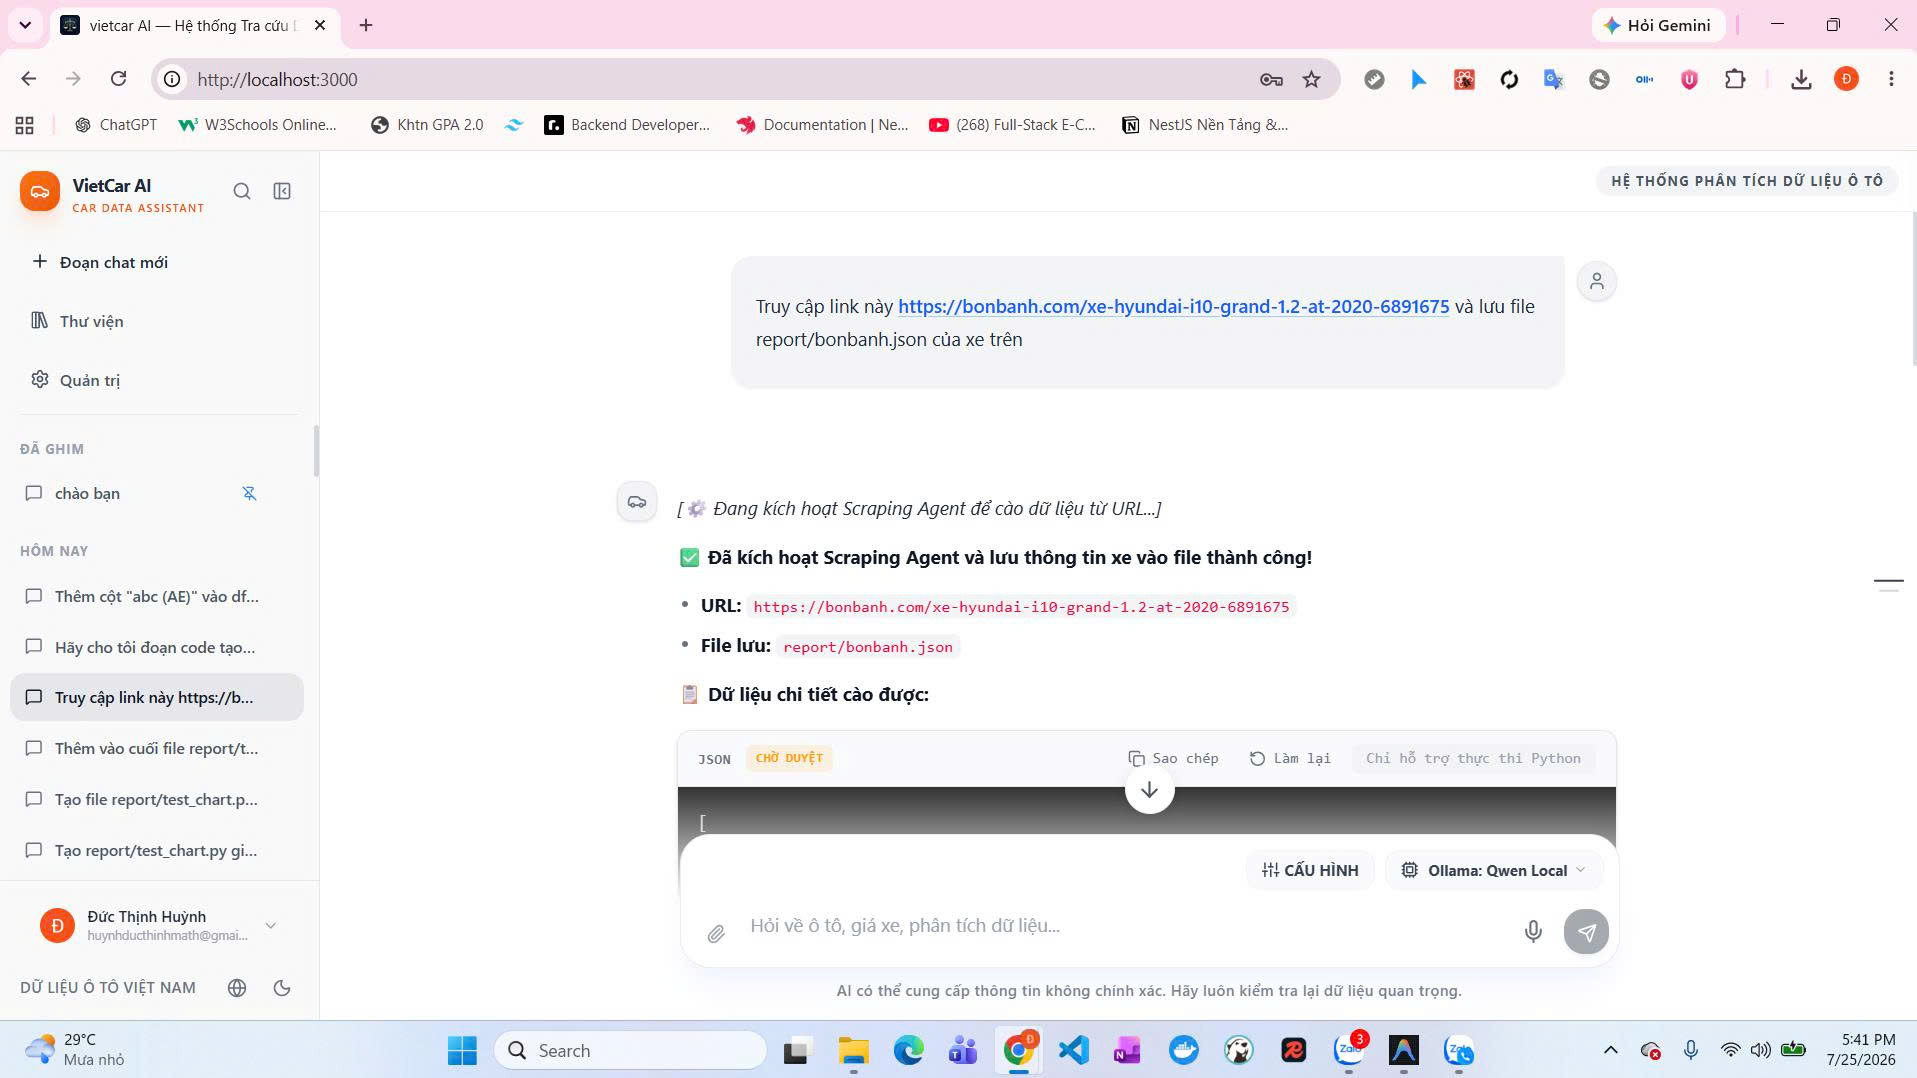
\includegraphics[width=1.00\textwidth]{graphics/AI/ai_tr92.jpg}
\caption{Phản hồi của AI sau khi Scraping Agent hoàn thành: thông báo đã lưu file thành công kèm đường dẫn, bảng thông số kỹ thuật xe được trích xuất (tên xe, năm, giá, nhiên liệu, hộp số, số km).}
\label{fig:ai_chat_overview}
\end{figure}


% ==============================================================================
% SUBSECTION 7: QUÁ TRÌNH SỬ DỤNG AI
% ==============================================================================
\subsection{Quá trình sử dụng AI trong đồ án}
\label{subsec:ai_usage_process}

Theo yêu cầu của hướng dẫn tích hợp AI (Mục 4), phần này tóm tắt quá trình nhóm sử dụng module AI để phân tích tập dữ liệu xe, bao gồm những yêu cầu đã đặt ra, kết quả đã nhận được và những thay đổi đã thực hiện trước khi chấp nhận kết quả.

% ------------------------------------------------------------------------------
\subsubsection{Những yêu cầu đã đặt ra}
\label{subsubsec:ai_requests}

Trong quá trình phân tích, nhóm đã đặt ra nhiều yêu cầu thuộc các nhóm chức năng khác nhau. Bảng dưới đây tổng hợp các nhóm yêu cầu tiêu biểu:

% Đừng quên thêm \usepackage{xltabular} vào preamble nếu bạn chưa có

\begin{xltabular}{\textwidth}{L{4.5cm} L{4.5cm} Y}
\caption{Các yêu cầu tiêu biểu đã đặt ra cho module AI trong quá trình phân tích}
\label{tab:ai_requests} \\
\hline
\textbf{Yêu cầu đặt ra} & \textbf{Công cụ AI sử dụng} & \textbf{Mục tiêu phân tích} \\ \hline
\endfirsthead

% Header lặp lại khi sang trang mới
\multicolumn{3}{c}%
{{\bfseries Bảng \thetable\ tiếp theo từ trang trước}} \\
\hline
\textbf{Yêu cầu đặt ra} & \textbf{Công cụ AI sử dụng} & \textbf{Mục tiêu phân tích} \\ \hline
\endhead

% Footer hiển thị ở cuối các trang bị ngắt
\hline \multicolumn{3}{r}{{Tiếp tục ở trang sau...}} \\
\endfoot

% Footer ở trang cuối cùng của bảng
\hline
\endlastfoot

% --- Nội dung bảng ---
Tính giá trung vị của xe theo từng hãng trong tập dữ liệu & \texttt{query\_dataset\_readonly} & Xác minh số liệu KPI Tab 2 (giá trung vị toàn thị trường = 638 triệu). \\
Thống kê số lượng xe điện theo từng năm sản xuất từ 2020 đến 2025 & \texttt{query\_dataset\_readonly} & Phân tích tốc độ tăng trưởng xe điện cho Tab 3. \\
Vẽ biểu đồ phân phối giá xe theo phân khúc (dưới 300 triệu, 300--600 triệu, ...) & \texttt{query\_dataset\_readonly} & Tạo biểu đồ kiểm chứng thiết kế dashboard Tab 2. \\
Kiểm tra phân bố tỷ lệ màu sắc ngoại thất trong tập dữ liệu & \texttt{query\_dataset\_readonly} & Xác minh số liệu biểu đồ màu xe Tab 4. \\
Đếm số xe Ford sản xuất năm 2023 & \texttt{query\_dataset\_readonly} & Kiểm chứng điểm đột biến nguồn cung được phát hiện ở Tab 5. \\
Xem thông số kỹ thuật của một mẫu xe Hyundai Kona từ bonbanh.com & \texttt{scrape\_car\_data} & Thu thập dữ liệu tham chiếu cho phần phân tích xe điện. \\
Sửa tiêu đề biểu đồ trong file \texttt{docs/test\_chart.py} & \texttt{modify\_file} & Cập nhật nội dung file script phân tích. \\
Xem lịch sử thay đổi của file \texttt{docs/test\_chart.py} & \texttt{show\_change\_history} & Kiểm tra các phiên bản đã được lưu sao lưu. \\
Hoàn tác file về một phiên bản cụ thể theo timestamp & \texttt{rollback\_last\_change} & Khôi phục nội dung file sau khi chỉnh sửa sai. \\

\end{xltabular}

% ------------------------------------------------------------------------------
\subsubsection{Kết quả đã nhận được}
\label{subsubsec:ai_results}

\noindent\textbf{Kết quả từ truy vấn dữ liệu (Tầng 3):}

Khi nhóm yêu cầu tính giá trung vị theo hãng, AI sinh ra đoạn code Pandas với giải thích rõ ràng, sau đó bảng kết quả được stream trực tiếp ra giao diện từ Python thực thi. Ví dụ kết quả tính số lượng xe điện theo năm (trích từ kết quả thực thi):

\begin{table}[H]
\centering
\small
\begin{tabular}{c c c}
\textbf{Năm sản xuất} & \textbf{Số tin đăng xe điện} & \textbf{Thị phần trong năm} \\ \hline
2020 & 17 & 0{,}32\% \\
2021 & 29 & 0{,}55\% \\
2022 & 134 & 2{,}91\% \\
2023 & 244 & 6{,}09\% \\
2024 & 104 & 4{,}50\% \\
2025 & 240 & 19{,}79\% \\
\end{tabular}
\caption{Ví dụ kết quả AI tính toán: số lượng và thị phần xe điện theo năm sản xuất (tính từ dữ liệu thực)}
\label{tab:ev_by_year_ai}
\end{table}

AI nhận xét ngắn bên dưới bảng: số liệu thị phần tăng từ dưới 1\% (năm 2020--2021) lên gần 20\% (năm 2025), phản ánh xu hướng tăng trưởng nhanh trong giai đoạn gần đây.

\noindent\textbf{Kết quả từ Interactive Code Execution:}
Khi nhóm yêu cầu vẽ biểu đồ phân phối giá, AI sinh ra đoạn code Matplotlib kèm giải thích. Sau khi nhóm kiểm tra, điều chỉnh màu sắc và nhãn trục, biểu đồ được thực thi và hiển thị inline ngay trong giao diện chat. Biểu đồ này sau đó được lưu ra file ảnh để đưa vào dashboard và báo cáo.
\begin{figure}[H]
\centering
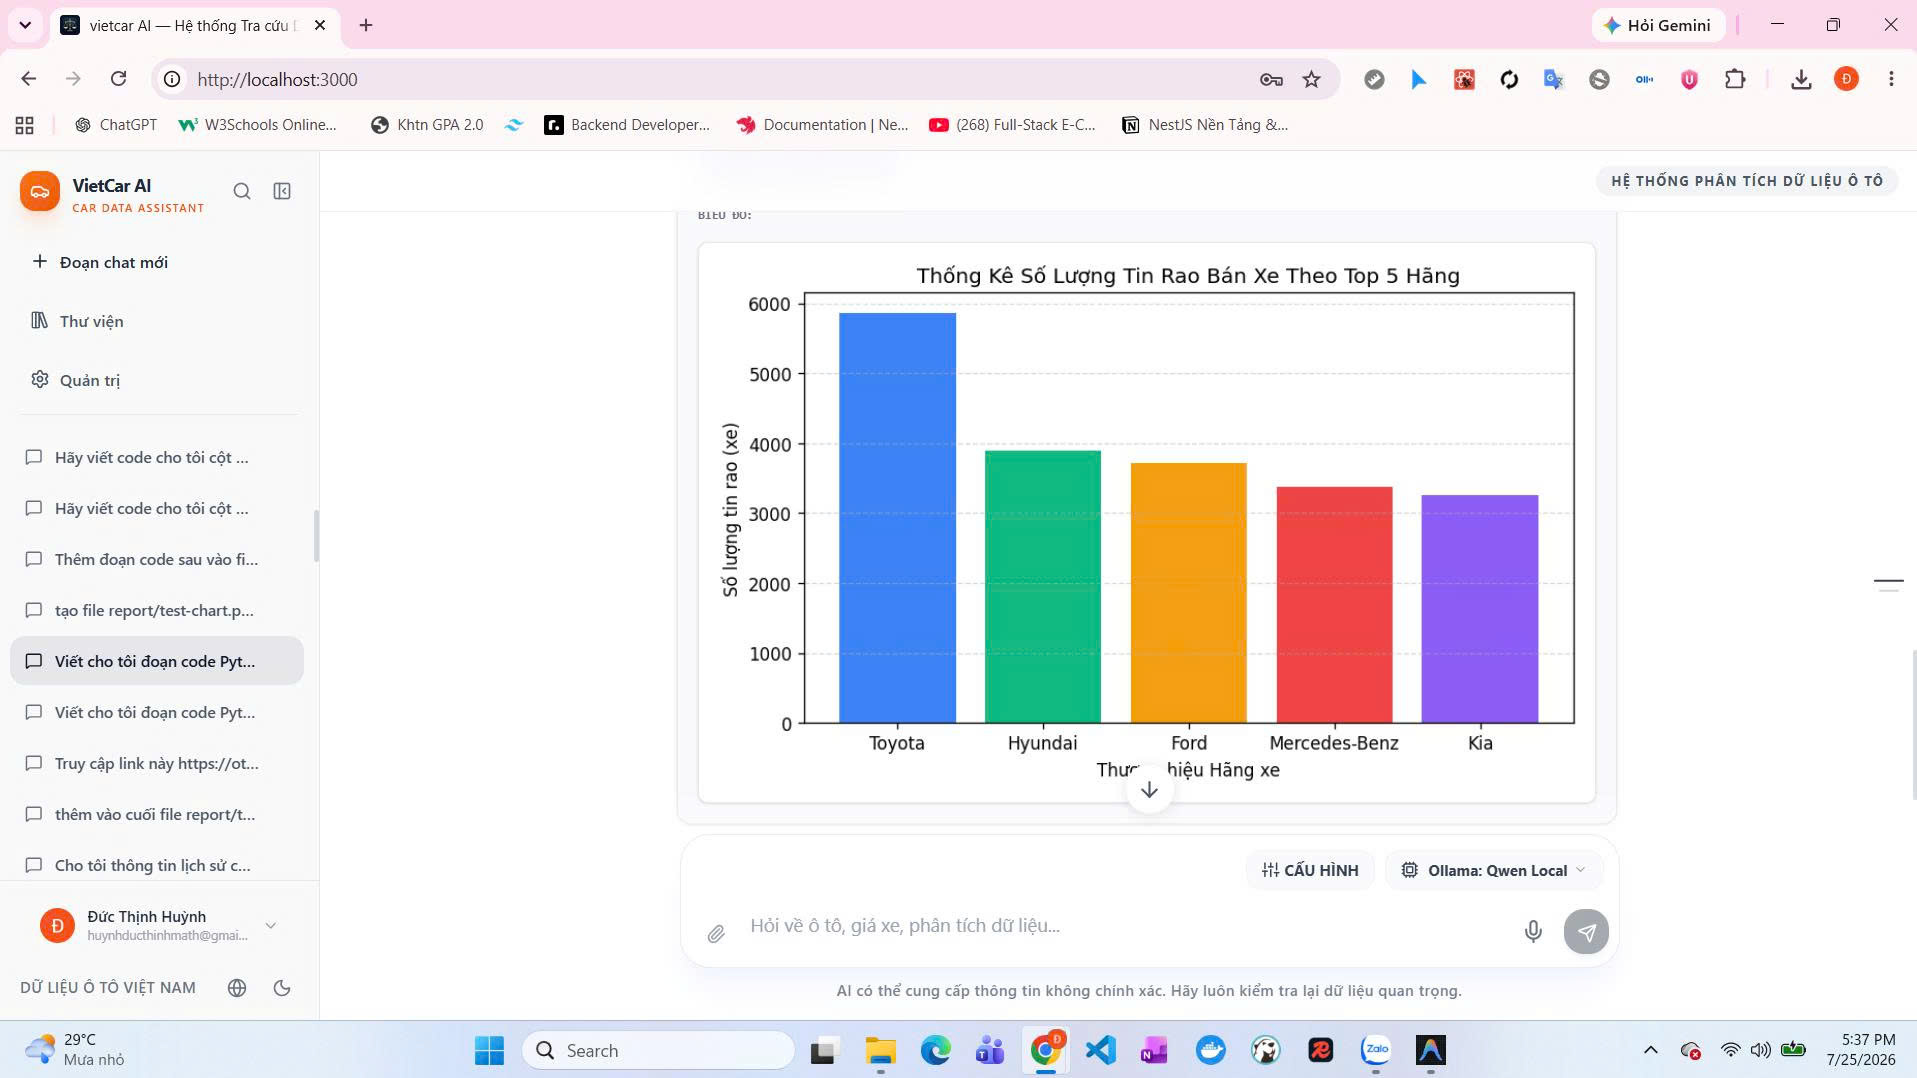
\includegraphics[width=1.00\textwidth]{graphics/AI/ai_tr82.jpg}
\caption{Kết quả thực thi code: biểu đồ phân phối giá xe hiển thị inline trong giao diện chat, phía trên là đoạn code Python đã thực thi, phía dưới là hình ảnh biểu đồ Matplotlib.}
\label{fig:ai_chat_overview}
\end{figure}

\noindent\textbf{Kết quả từ Scraping Agent:}
Khi nhóm cung cấp URL một tin đăng xe, Scraping Agent thu thập được đầy đủ thông tin bao gồm: tên xe, hãng, năm sản xuất, giá, nhiên liệu, hộp số, số km đã đi, màu sắc và các thông số kỹ thuật liên quan. Kết quả được lưu ra file JSON theo yêu cầu và hiển thị trực tiếp trên giao diện.

% ------------------------------------------------------------------------------
\subsubsection{Những thay đổi đã thực hiện}
\label{subsubsec:ai_changes}

Trong phần lớn các trường hợp, nhóm đã can thiệp vào đoạn code AI sinh ra trước khi thực thi. Bảng dưới đây ghi lại các loại thay đổi phổ biến:

% Nhớ thêm \usepackage{longtable} vào preamble

{\small
\begin{longtable}{p{4cm} p{3.5cm} p{7.5cm}}
\caption{Các loại thay đổi nhóm thực hiện trên đoạn code AI sinh ra trước khi chấp nhận}
\label{tab:ai_changes} \\
\hline
\textbf{Loại thay đổi} & \textbf{Ví dụ cụ thể} & \textbf{Lý do điều chỉnh} \\ \hline
\endfirsthead

% Cấu hình phần đầu bảng (header) nếu bảng bị tràn sang trang thứ 2
\multicolumn{3}{c}%
{{\bfseries Bảng \thetable\ tiếp theo từ trang trước}} \\
\hline
\textbf{Loại thay đổi} & \textbf{Ví dụ cụ thể} & \textbf{Lý do điều chỉnh} \\ \hline
\endhead

% Cấu hình phần chân bảng (footer) ở các trang bị ngắt
\hline \multicolumn{3}{r}{{Tiếp tục ở trang sau...}} \\
\endfoot

% Cấu hình phần chân bảng ở trang cuối cùng
\hline
\endlastfoot

% --- Nội dung bảng ---
Thay đổi tham số lọc & Đổi ngưỡng lọc xe đời mới từ năm 2020 sang năm 2018 & Bao quát giai đoạn phân tích rộng hơn theo yêu cầu đồ án. \\
Điều chỉnh màu biểu đồ & Đổi \texttt{color=`blue'} sang palette tông xanh lục đồng nhất với dashboard & Đảm bảo nhất quán về màu sắc với thiết kế Power BI. \\
Thêm nhãn dữ liệu & Thêm \texttt{plt.bar\_label()} để hiển thị giá trị trực tiếp lên thanh cột & Biểu đồ gốc AI sinh ra chưa có nhãn số liệu trên các thanh. \\
Sửa tên cột & Đổi tên cột từ \texttt{`Hang'} sang \texttt{`Hãng'} do không khớp tên cột thực & AI sử dụng tên cột sai dẫn đến lỗi \texttt{KeyError}. \\
Thu hẹp tập dữ liệu & Thêm điều kiện \texttt{df[df[`Tình trạng'] == `Xe đã dùng']} & Chỉ muốn phân tích riêng nhóm xe cũ, không phải toàn bộ. \\
Từ chối thao tác file & Bấm ``Từ chối'' khi AI đề xuất xóa file \texttt{docs/test.py} & Nhóm xác nhận file đó vẫn cần giữ lại cho bước phân tích tiếp theo. \\
Rollback phiên bản file & Yêu cầu hoàn tác \texttt{docs/test\_chart.py} về bản backup cụ thể & Sau khi sửa tiêu đề biểu đồ, nhận ra bản gốc phù hợp hơn. \\

\end{longtable}
}

% ==============================================================================
% SUBSECTION 8: NHẬN XÉT VỀ AI
% ==============================================================================
\subsection{Nhận xét về module AI}
\label{subsec:ai_review}

Sau quá trình xây dựng và sử dụng module AI trong đồ án, nhóm rút ra một số nhận xét về ưu điểm, hạn chế và bài học kinh nghiệm như sau.

\subsubsection{Ưu điểm quan sát được}
\label{subsubsec:ai_pros}

\begin{itemize}
    \item \textbf{Tốc độ phản hồi linh hoạt theo loại câu hỏi:} Kiến trúc 3 tầng cho phép hệ thống phản hồi gần như tức thì với câu hỏi tổng quan (Tầng 1) trong khi vẫn đảm bảo độ chính xác với câu hỏi tính toán cụ thể (Tầng 3). Người dùng không cần phân biệt rõ loại câu hỏi; hệ thống tự nhận diện và chọn đường xử lý phù hợp.

    \item \textbf{Số liệu từ dữ liệu thực, ít xảy ra nhầm lẫn số liệu:} Do số liệu trong phản hồi của AI luôn đến từ kết quả thực thi Pandas trên tập CSV gốc, hiện tượng AI tự sáng tác con số được kiểm soát tốt hơn so với hướng tiếp cận để LLM tự trả lời câu hỏi định lượng.

    \item \textbf{Linh hoạt về nhà cung cấp LLM:} Hệ thống hỗ trợ chuyển đổi giữa Groq (nhanh), OpenAI, Google và Ollama (chạy local không cần internet) mà không cần thay đổi code. Điều này giúp nhóm thử nghiệm và so sánh chất lượng phản hồi giữa các mô hình.

    \item \textbf{Giao diện InteractiveCodeBlock trực quan:} Người dùng có thể đọc, sửa và thực thi code trong cùng một giao diện, giảm bước chuyển qua môi trường ngoài. Biểu đồ Matplotlib hiển thị ngay inline trong chat mà không cần lưu file ảnh thủ công.

    \item \textbf{Cơ chế backup và rollback an toàn:} Việc tự động sao lưu trước mỗi thao tác ghi đã giúp nhóm khôi phục lại file về trạng thái mong muốn trong một số trường hợp chỉnh sửa sai mà không mất dữ liệu.
\end{itemize}

\subsubsection{Hạn chế quan sát được}
\label{subsubsec:ai_cons}

\begin{itemize}
    \item \textbf{Phân loại intent đôi khi chưa chính xác:} Bộ phát hiện intent dựa trên từ khóa nên một số câu hỏi có từ khóa mơ hồ có thể bị định tuyến sai tầng. Ví dụ, câu hỏi ``Tôi muốn viết code sửa file dữ liệu'' đôi khi bị nhận nhầm là yêu cầu tính toán dữ liệu thay vì yêu cầu quản lý file.

    \item \textbf{Mô hình local (Ollama) có chất lượng phản hồi chưa ổn định:} Khi sử dụng mô hình nhỏ chạy local như Llama 3.2 3B, chất lượng giải thích code và khả năng nhận diện ngữ cảnh tiếng Việt kém hơn đáng kể so với mô hình đám mây. Một số câu hỏi phức tạp cần phải đặt lại hoặc diễn đạt đơn giản hơn.

    \item \textbf{Scraping Agent phụ thuộc vào cấu trúc trang web:} Nếu trang bonbanh.com thay đổi cấu trúc HTML hoặc bổ sung cơ chế chống bot, script cào dữ liệu cần được cập nhật tương ứng. Tính năng này hoạt động tốt tại thời điểm xây dựng nhưng có thể cần bảo trì trong tương lai.

    \item \textbf{Thời gian thực thi tác vụ cào dữ liệu tương đối dài:} Scraping Agent cần tải và render trang web đầy đủ nên mỗi lần cào một URL mất từ 15 đến 60 giây tùy tốc độ mạng và độ phức tạp của trang.

    \item \textbf{Giải thích code chưa đồng đều:} Một số mô hình LLM sinh ra giải thích quá ngắn gọn hoặc dùng thuật ngữ kỹ thuật mà người dùng không chuyên có thể khó hiểu. Chất lượng giải thích phụ thuộc khá nhiều vào mô hình được chọn.
\end{itemize}

\subsubsection{Bài học kinh nghiệm}
\label{subsubsec:ai_lessons}

\begin{itemize}
    \item \textbf{Kiểm tra trước khi thực thi:} Kinh nghiệm thực tế cho thấy việc đọc kỹ đoạn code AI sinh ra trước khi bấm Thực thi giúp phát hiện kịp thời các trường hợp AI dùng tên cột sai hoặc điều kiện lọc chưa đúng với mục tiêu phân tích.

    \item \textbf{Diễn đạt câu hỏi cụ thể hơn cho kết quả tốt hơn:} Câu hỏi càng cụ thể (ghi rõ tên cột, điều kiện lọc, khoảng thời gian) thì code AI sinh ra càng gần với ý định và ít cần chỉnh sửa hơn. Câu hỏi mơ hồ thường dẫn đến code tổng quát và cần nhiều vòng điều chỉnh.

    \item \textbf{Tận dụng khả năng đề xuất hướng phân tích:} Khi nhóm chưa có ý tưởng về cách tiếp cận một câu hỏi phân tích, việc yêu cầu AI liệt kê các hướng phân tích có thể thực hiện với tập dữ liệu đã tiết kiệm thời gian đáng kể so với tìm kiếm tài liệu từ đầu.

    \item \textbf{Xác nhận số liệu quan trọng từ nhiều nguồn:} Với các con số được đưa vào kết luận chính thức trong báo cáo, nhóm thực hiện kiểm tra chéo bằng cách chạy lại truy vấn với cách viết code khác nhau hoặc đối chiếu với kết quả từ Power BI để đảm bảo tính nhất quán.
\end{itemize}

\clearpage
